\documentclass[a4paper]{article}

\usepackage[english]{babel}
\usepackage[utf8]{inputenc}
\usepackage{amsmath}
\usepackage{graphicx}
\usepackage[colorinlistoftodos]{todonotes}
\usepackage{hyperref}
\usepackage{listings}
\usepackage[numbers]{natbib}

\usepackage{booktabs} % To thicken table lines



\title{Building a Student Intervention System}

\author{Uirá Caiado}

\date{\today}

\begin{document}

\maketitle

\begin{abstract}
% it is a comment. Pretty nice, hum 
There exists a push from educators and administrators to raise the likelihood of students successfully complete their programs. The aim of this project is to identify students who need intervention before they drop out of school. My goal is to use concepts from supervised machine learning to find the most effective model with the least amount of computation costs that identify such students.
\end{abstract}

%%%%%%%%%%%%%%%%%%%%%%%%%%%%%%%%%%%%%%%%%%%%%%%%%%%%%%%%%%%%%%%%%%%%%%%%%%%%%%%%%%%%%%%%
%% INTRODUCTION
%%%%%%%%%%%%%%%%%%%%%%%%%%%%%%%%%%%%%%%%%%%%%%%%%%%%%%%%%%%%%%%%%%%%%%%%%%%%%%%%%%%%%%%%

\section{Introduction}
\label{sec:introduction}

% https://goo.gl/i8TQwZ: shorten url for https://www.udacity.com/course/viewer%5C#!/c-nd009/l-5446988865/m-5446493941

\subsection{Some Background}
As stated by Udacity\footnote{Source: \url{https://goo.gl/i8TQwZ}} in the description for this project, as education has grown to rely more and more on technology, more and more data is available for examination and prediction. Logs of student activities, grades, interactions with teachers and fellow students, and more are now captured through learning management systems.

Within all levels of education, there exists a surge to help increase the likelihood of student success without watering down the education or engaging in behaviors that raise the probability of passing metrics without improving the actual underlying learning. Graduation rates are often the criteria of choice for this, and educators and administrators are after new ways to predict success and failure early enough to stage effective interventions, as well as to identify the effectiveness of different interventions.

\subsection{The Goal}
The goal for this project is implementing a student intervention system using concepts from Supervised Machine Learning. I am going to choose and develop a model that will predict the likelihood that a given student will pass, thus helping diagnose whether or not an intervention is necessary.

I will suppose that the data available to create the model is a representative but a small sample of the dataset that I would have access in the production environment. So, besides the typical accuracy requirements for any machine-learning project, I am also going to look for models that are efficient in the use of resources (computation time and memory). Thus, the model will be evaluated on three factors:

\begin{itemize}
\item Its $F_1$\footnote{Source: \url{https://en.wikipedia.org/wiki/F1_score}} Score, summarizing the number of correct positives and correct negatives out of all possible cases. In other words, how well does the model differentiate likely passes from failures
\item The size of the training set, preferring smaller training sets over larger ones. That is, how much data does the model need to make a reasonable prediction?
\item The computation resources to make a reliable prediction. How much time and memory is required to correctly identify students that need intervention?
\end{itemize}

\subsection{Classification vs Regression}
The model that will be developed is a Classifier. According to \cite{Hastie_2009}, the distinction in the output type has led to a naming convention for prediction tasks: \textit{regression} when we predict quantitative (continuous) outputs, and \textit{classification} when we predict qualitative outputs (discrete). As the goal of this project is to identify if the student will succeed, the problem posed is a classification problem once it requires a binary answer (passed, failed).

%%%%%%%%%%%%%%%%%%%%%%%%%%%%%%%%%%%%%%%%%%%%%%%%%%%%%%%%%%%%%%%%%%%%%%%%%%%%%%%%%%%%%%%%
%% EXPLORING THE DATA
%%%%%%%%%%%%%%%%%%%%%%%%%%%%%%%%%%%%%%%%%%%%%%%%%%%%%%%%%%%%%%%%%%%%%%%%%%%%%%%%%%%%%%%%


\section{Exploring the Data}
\label{sec:exploring_data}
In this section, we will explore the data to look for insides about the features.

\subsection{Basic Facts}
Let's go ahead and execute a basic description of the student dataset (Table \ref{tab:basicfacts}):

\begin{table}[ht]
\centering
\begin{tabular}{l|r}
 & Value \\\hline
Total number of students & 42 \\
Total number of students & 395 \\
Number of students who passed & 265 \\
Number of students who failed & 130 \\
Number of features & 31 \\
Graduation rate of the class & 67.09 \%

\end{tabular}
\caption{\label{tab:basicfacts}Facts About the Dataset.}
\end{table}

% https://goo.gl/dkHKPV: shorten url for https://github.com/udacity/machine-learning/tree/master/projects/student_intervention
All the 31 features in the dataset are discrete and Qualitative. There are 14 binary data, 13 ordered categorical variables and other 4 Categorical features. Among them, there are variables such as Father's Job, Family Size, if the student wants to take higher education or if he/she is in a romantic relationship. The data offers a pretty comprehensive profile of student life. At this point, it is hard to say what features are relevant or not. A complete description of each variable can be found on the Github project page\footnote{Source: \url{https://goo.gl/dkHKPV}}. There is no missing data on this dataset and no presence of ``real'' outliers.

\subsection{How the features are spread out}
Before moving on, I am going to plot each feature to see how each inner classes of each variable are divided between the target labels ``Passed'' and ``Not Passed''. In the Figure~\ref{fig:categorical} is plotted the Categorical features of the dataset. Here is possible to see that when the guardian is not the mother nor the father, it is more likely that the pupil not pass. Also, when the mother's occupatsion is teaching (\textit{Fjob}), is likely that the student to pass.

\begin{figure}[ht]
\centering
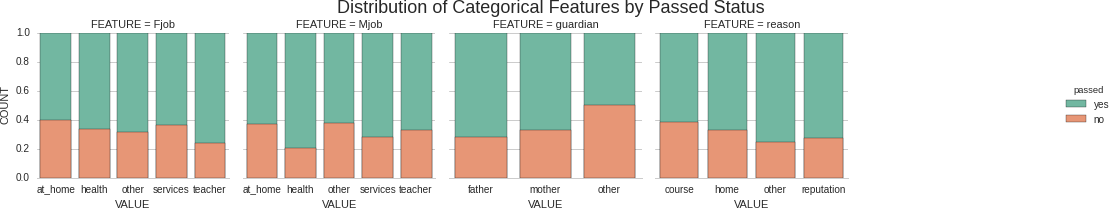
\includegraphics[width=0.75\textwidth]{figures/categorical.png}
\caption{\label{fig:categorical}Categorical Data.}
\end{figure}

Looking at the Ordered Categorical Features (Figure~\ref{fig:ordCategorical}), where there is an ordering of the values, the features \textit{absences}, \textit{age} and \textit{failure} stand out. The \textit{failures} feature is the number of past class failures ($n$ if $1<=n<3$, else $4$) and absences is the number of school absences. In all these variables, the bigger the number, the higher the likelihood of the student does not pass.

\begin{figure}[ht]
\centering
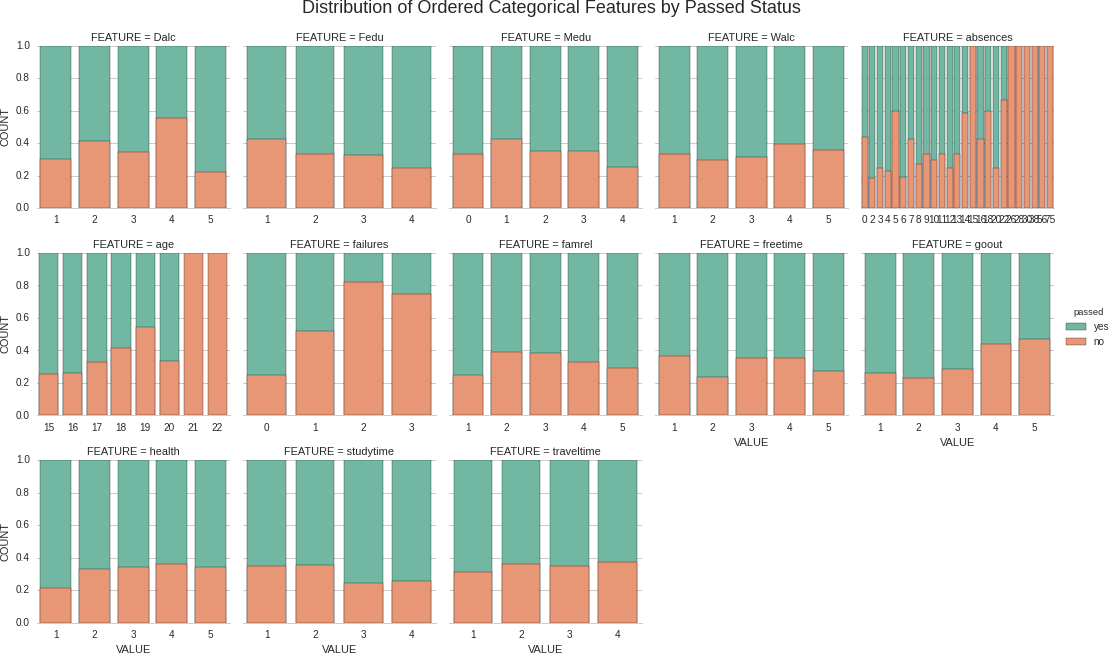
\includegraphics[width=0.75\textwidth]{figures/ordCategorical.png}
\caption{\label{fig:ordCategorical}Ordered Data.}
\end{figure}

Finally, looking at the Binary Data (Figure~\ref{fig:binary}), what more draw the attention are the features \textit{higher} and \textit{schoolsup}. The feature \textit{higher} is if the student wants to take higher education and \textit{schoolsup} is if the student has extra educational support. Some features, as \textit{activities} and \textit{nursery}, presented a very similar distribution between the classes

\begin{figure}[ht]
\centering
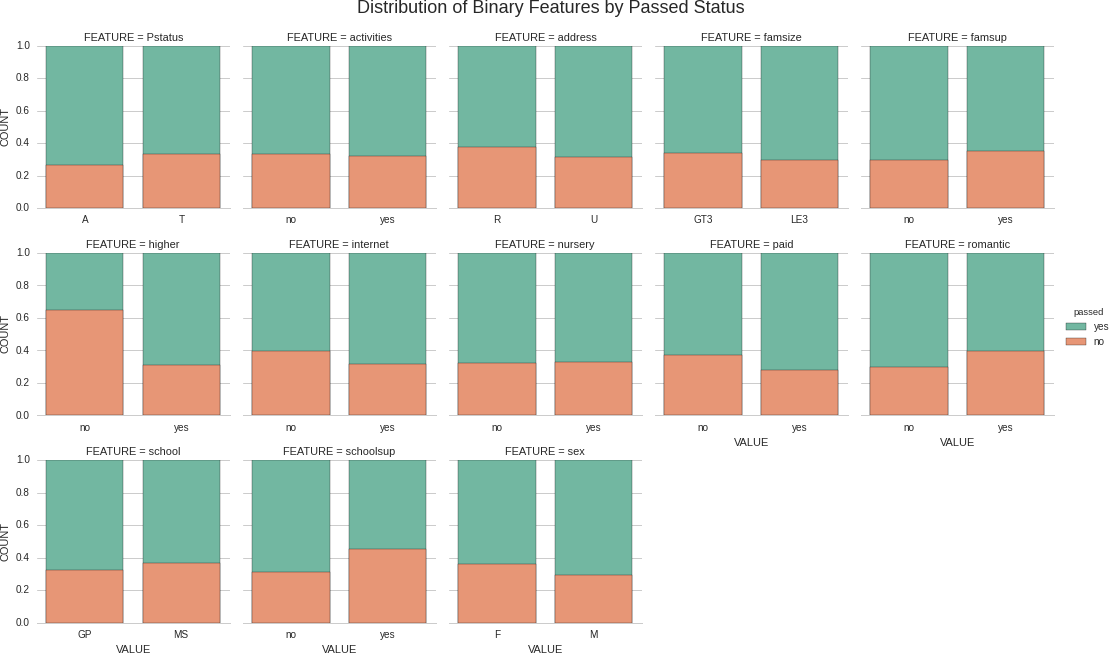
\includegraphics[width=0.75\textwidth]{figures/binary.png}
\caption{\label{fig:binary}Binary Data.}
\end{figure}

As can be seen, there are a lot of features that might add up to the classification process, although some features may be not so relevant It is important to notice that the model developed with this amount of data (365 data points) and variables (31) can suffer from the  \textit{curse of dimensionality}\footnote{Source: \url{https://en.wikipedia.org/wiki/Curse_of_dimensionality}}. Many of the features will be converted into dummy variables, what could increase the amount of data needed to build an accurate model.

%%%%%%%%%%%%%%%%%%%%%%%%%%%%%%%%%%%%%%%%%%%%%%%%%%%%%%%%%%%%%%%%%%%%%%%%%%%%%%%%%%%%%%%%
%% PREPARING THE DATA
%%%%%%%%%%%%%%%%%%%%%%%%%%%%%%%%%%%%%%%%%%%%%%%%%%%%%%%%%%%%%%%%%%%%%%%%%%%%%%%%%%%%%%%%

\section{Preparing the Data}
In this section, I will prepare the data for modeling, training and testing.
\subsection{Identify feature and target columns}
It is often the case that the data you obtain contains non-numeric features. This can be a problem, as most machine learning algorithms expect numeric data to perform computations with.

% code snipet
\begin{lstlisting}
Feature column(s):
===================
school         	sex            	age            	address        
famsize        	Pstatus        	Medu           	Fedu           
Mjob           	Fjob           	reason         	guardian       
traveltime     	studytime      	failures       	schoolsup      
famsup         	paid           	activities     	nursery        
higher         	internet       	romantic       	famrel         
freetime       	goout          	Dalc           	Walc           
health         	absences       

Target column:
===================
passed

Feature values:
===================
  school sex  age address famsize Pstatus  Medu  Fedu
0     GP   F   18       U     GT3       A     4     4
1     GP   F   17       U     GT3       T     1     1
2     GP   F   15       U     LE3       T     1     1
3     GP   F   15       U     GT3       T     4     2
4     GP   F   16       U     GT3       T     3     3 ...
\end{lstlisting}

\subsection{Preprocess feature columns}
As can be seen above, there are several non-numeric columns in the dataset that need to be converted. The easiest case is when are only two categories, as ``yes'' or ``no'', e.g. \textit{internet}. These are often represented by single binary digit as $0$ or $1$.

According to \cite{Hastie_2009}, when there are more than two categories, the most commonly alternative used is coding via \textit{dummy variables}\footnote{Source: \url{https://www.moresteam.com/whitepapers/download/dummy-variables.pdf}}. This method consists in representing a $K$-Level qualitative variable by a vector of $K$ binary variables, where only one of which is ``on'' at a time.

So, for example, the \textit{Fjob} feature will be split into $5$ new features ( \textit{Fjob\_teacher}, \textit{Fjob\_other}, \textit{Fjob\_services}, etc.), and will be assigned a $1$ to one of them and $0$ to all other columns.

This transformation will be performed using the pandas function `get\_dummies()`. Initially, all binary data that the classes do not correspond to $yes$/$no$ will be converted into dummies.

% insert code snippet
\begin{lstlisting}
Processed feature columns (48):
===================

school_GP         	school_MS         	sex_F             
sex_M             	age               	address_R         
address_U         	famsize_GT3       	famsize_LE3       
Pstatus_A         	Pstatus_T         	Medu              
Fedu              	Mjob_at_home      	Mjob_health       
Mjob_other        	Mjob_services     	Mjob_teacher      
Fjob_at_home      	Fjob_health       	Fjob_other        
Fjob_services     	Fjob_teacher      	reason_course     
reason_home       	reason_other      	reason_reputation 
guardian_father   	guardian_mother   	guardian_other    
traveltime        	studytime         	failures          
schoolsup         	famsup            	paid              
activities        	nursery           	higher            
internet          	romantic          	famrel            
freetime          	goout             	Dalc              
Walc              	health            	absences  
\end{lstlisting}

\subsection{Split data into training and test sets}
So far, I have converted all \textit{categorical} features into numeric values. To be able to judge if the model chosen in the next section will generalize well from its experience, I will hold out part of the data to measure how the algorithms are performing on yet-unseen examples. In this next step, I am going to split the data (both features and corresponding labels) into training and test sets. I will use the function \textit{cross\_validation.train\_test\_split()} from \textit{scikit-learn} for that.

\begin{lstlisting}
Training set: 296 samples
Test set: 99 samples
\end{lstlisting}

%%%%%%%%%%%%%%%%%%%%%%%%%%%%%%%%%%%%%%%%%%%%%%%%%%%%%%%%%%%%%%%%%%%%%%%%%%%%%%%%%%%%%%%%
%% TRAINING AND EVALUATING THE MODELS
%%%%%%%%%%%%%%%%%%%%%%%%%%%%%%%%%%%%%%%%%%%%%%%%%%%%%%%%%%%%%%%%%%%%%%%%%%%%%%%%%%%%%%%%

\section{Training and Evaluating Models}
As stated in Section 1, the model will be evaluated on three factors: $F_1$ Score, The size of the training set needed to build an acceptable model, and the computation resources used. Before selecting the algorithms to test their performance and amount of data needed, I am going to check the resources that different Supervised Learning Algorithms take by training them using different sizes of data sets.  After that, I will select three algorithms to describe and analyze their performance under different training set sizes using their learning curves

\subsection{Computation Resources Test}
I am going to test computation resources needed for six different algorithms: $Decision Tree$, $SVM$, $K-NN$, $Naive Bayes$, $Logistic Regression$ and $AdaBoost$. I will use the scikit-Learn implementation of these algorithms using their default parameters.

To assess more realistic measurements of the resources used, I will create new datasets with the training and test datasets repeated 8 times. In the next subsection, where I will check the $F_1$ score of some of these models, I will perform the tests again using the original data.

In the Figure~\ref{fig:timetest}, I have measured the time that each algorithm took to fit the model and to perform the predictions. As expected, $K-NN$ took longer in the testing phase than in the training phase. As instead of  fit a model to the data, it holds the examples to find the closest neighbors, this behavior was expected. 

The $SVM$ presented a curious behavior. The time increased sharply and dropped suddenly. As pointed out in the scikit documentation\footnote{Source: \url{http://scikit-learn.org/stable/modules/svm.html\#complexity}}, the fit time complexity of the SVM is more than quadratic.

\begin{figure}[ht!]
\centering
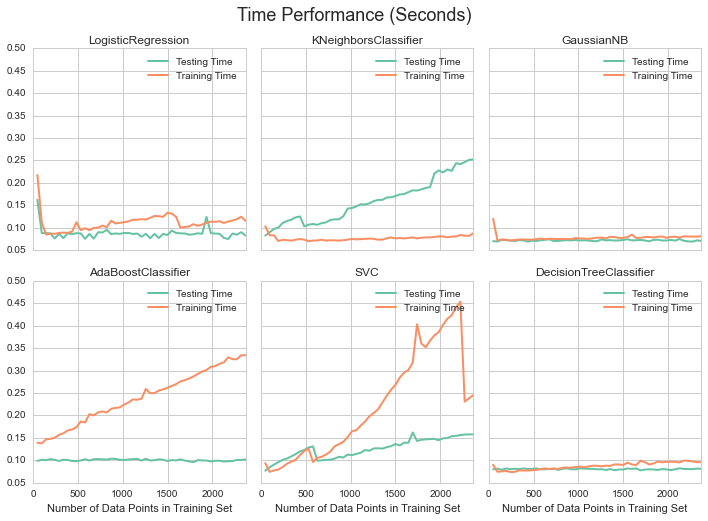
\includegraphics[width=0.75\textwidth]{figures/timePerformance.png}
\caption{\label{fig:timetest}Time Performance of different algorithms}
\end{figure}

% http://goo.gl/QR1gB8: http://stackoverflow.com/questions/22397485/what-is-the-o-runtime-complexity-of-adaboost
The time complexity of the $AdaBoost$ Classifier depends on the number of base learners\footnote{Source: \url{http://goo.gl/QR1gB8}} used ($Decision Tree$ and the maximum 50, respectively). The time to fit the model has increased with more data, although the time to predict was kept at an acceptable level.

Considering the resources constraints, I will keep testing just the models that presented a relatively stable time both to test and to predict. In the next section, I will analyze the $F_1$ score of the $Gaussian Naive Bayes$, $Decision Tree$ and $Logistic Regression$.

\subsection{Performance Test}

In this subsection, I will analyze each model chosen in the last section, presenting a brief explanation about each one and examining its learning curves.

\subsubsection{Naive Bayes}
According to \cite{Mitchell}, one highly piratical Bayesian learning method is the naive Bayes learner. Its performance has been shown to be comparable to neural network and decision tree learning in some domains. The model assumes that each feature is conditionally independent given a target value:

$$\upsilon_{NB} = \arg\max_{v_j \in V}P(\upsilon_j) \prod_i P(a_i | \upsilon_j) $$

Where $\upsilon_{NB}$ is the label (passed or not passed, in this case) that maximize this calculation. The model classifies any data point by multiplying the probability of a particular class and the likelihood of observing each feature given that class.

\cite{Hastie_2009} says that, while the model assumption is generally not true, it does simplify the estimation drastically. it also indicates that the probability of a given event probability might be wrong, but the conclusion will be right.

In the Figure~\ref{fig:gaussianNB} is possible to see that the $F_1$ score has stabilized already around 100 data points used to fit the model, but its maximum score it achieved just around 296 data points. The training and test time are pretty close, as shown in the Figure~\ref{fig:timetest}.

\begin{figure}[ht!]
\centering
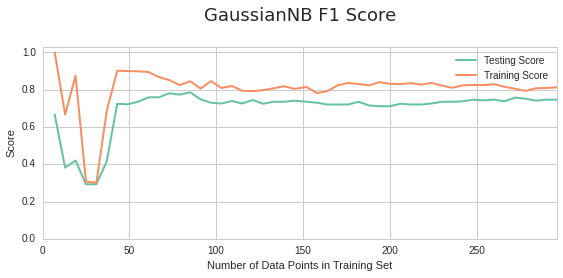
\includegraphics[width=0.75\textwidth]{figures/guassianNB.png}
\caption{\label{fig:gaussianNB}Naive Bayes Learning Curve}
\end{figure}

\begin{table}[ht!]
\centering
\begin{tabular}{l|rrr}
{} & \multicolumn{3}{ c }{Training set size }         \\
{} &               103 &     200 &     296 \\\hline
prediction time (secs)   &            0.0889 &  0.0801 &  0.0890 \\
training time (secs)     &            0.0708 &  0.0862 &  0.0803 \\
F1 score on test set     &            0.7259 &  0.7111 &  0.7465 \\
F1 score on training set &            0.8092 &  0.8315 &  0.8120 \\
\end{tabular}
\caption{\label{tab:NayveBayes}Nayve Bayes Measurements}
\end{table}


The sklearn documentation\footnote{Source: \url{http://scikit-learn.org/stable/modules/naive_bayes.html}} states that  one of the common use of the algorithm is in classification and spam filtering. The model requires a small amount of training data to estimate the necessary parameters.

Some of the pros of this model are: inference is cheap; the model has few parameters; empirically successful. A negative side is that The assumption that the attributes be conditional independent of each other is too strong. For example, it can't learn interactions between labels\footnote{Source: \url{http://blog.echen.me/2011/04/27/choosing-a-machine-learning-classifier/}}.

Given the resource consumption of the Naive Bayes to train and predict and the $F_1$ Score achieved, this model seems a strong candidate for the final model.

\subsubsection{Decision Tree}

\cite{Mitchell} explained that Decision tree is a method for approximating discrete-valued functions that are robust to noisy data and capable of learning disjunctive expressions. The model classifies instances by sorting them down the tree from the root to some leaf node (which is the label of the data).  It has been applied to a broad range of tasks from learning to diagnose medical cases to learning to assess credit risk of loan applicants.

The \textit{Scikit-learn} uses an optimized version of the CART (Classification and regression trees) algorithm, that basically constructs binary trees using the feature and threshold that yield the largest information gain at each node. So, as shown by \cite{Hastie_2009}, given that there are 2 classes in the dataset (or regions $R_1$ and $R_2$):

$$f(x) = \sum_{m=1}^2 c_m I(x \in R_m)$$

Where:
\begin{itemize}
\item $\hat{c}_m = ave(y_i|x_i \in R_m)$
\item $R_1 (j,s) = \{ X | X_{j}<s\}$ and $R_2 (j,s) = \{ X | X_{j}>s\}$
\end{itemize}

$I(.)$ is an indicator function\footnote{Source: \url{https://en.wikipedia.org/wiki/Indicator_function}} and $\hat c$ is what should be minimized by tweaking the combination of the splitting feature and the split point $(j,s)$. The procedure to minimize $\hat c$ can be found in \textit{Scikit-learn} documentation\footnote{Source: \url{http://scikit-learn.org/stable/modules/tree.html\#tree}}.

The figure ~\ref{fig:DT} shows clearly that the model overfits the Training Data set, although it seems that didn't affect the $F_1$ score in the test set. Instead, it continues to grow significantly when more data is added. The time to train and test is similar to the $GaussianNB$ results.

\begin{figure}[ht!]
\centering
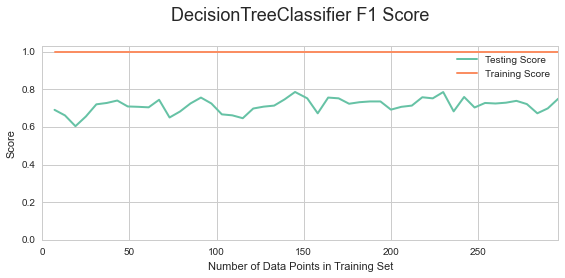
\includegraphics[width=0.75\textwidth]{figures/DT.png}
\caption{\label{fig:DT}Decision Tree Learning Curve}
\end{figure}

\begin{table}[ht!]
\centering
\begin{tabular}{l|rrr}
{} & \multicolumn{3}{ c }{Training set size }         \\
{} &               103 &     200 &     296 \\\hline
prediction time (secs)   &            0.0888 &  0.0788 &  0.0924 \\
training time (secs)     &            0.0767 &  0.0818 &  0.0842 \\
F1 score on test set     &            0.6667 &  0.6917 &  0.7500 \\
F1 score on training set &            1.0000 &  1.0000 &  1.0000 \\
\end{tabular}
\caption{\label{tab:DT}Decision Tree Measurements}
\end{table}

Still according to the documentation, some advantages of decision trees are: Decision Trees are simple to understand and to interpret, as they can be visualized; Requires little data preparation (like normalization); Performs well even if its assumptions are somewhat violated by the true model; The cost of using the tree is logarithmic in the number of data points used in the training phase.

The disadvantages include: it can create over-complex trees that do not generalize the data well; and if some classes dominate,the tree can be biased. Many disadvantages of this algorithm is mitigated by using decision trees within an ensemble, like $AdaBoost$.

An advantage of the $Decision Tree$ algorithm over the $GuassianNB$ is that it could be visualized, what would make it easier to explain to someone without knowledge about Machine Learning. However, It took more data to fit a similar model regarding $F_1$ score when compared to the last method. Also, this particular dataset is imbalanced (there are 60\% of passed and 30\% of not passed), and it can be an issue. Using the model within an ensemble method, as suggest in the last paragraph, is not feasible given the time to train the model, as shown in the Figure~\ref{fig:timetest}.

\subsubsection{Logistic Regression}
Contrary to its name, logistic regression is a classification method that performs a regression in a logistic (or sigmoid)\footnote{Source: \url{https://en.wikipedia.org/wiki/Generalised_logistic_function}} function , as said in \cite{richert2013building}. In \cite{Hastie_2009} book is said that this model is widely used in biostatistical applications where binary responses occur quite frequently. For instance, patients survive or die, have heart disease or not and so on. This model is usually fit by maximum likelihood, using the conditional probability of $G$ given $X$. The general log-likelihood that should be maximized to $\theta$(that will result in the $\beta$ parameters of the function) is:

$$l(\theta) = \sum_{i=1}^{N} \log{p_{g_{i}}(x_i; \theta)}$$

% http://goo.gl/T7h0Hz: shorten for http://scikit-learn.org/stable/modules/linear_model.html\#logistic-regression
Where $p_{k}(x_i ; \theta) = Pr(G=k | X = x_i ; \theta)$ and the probabilities sum up to 1. The default implementation of \textit{Scikit-Learn }solves the maximization problem using the C++ library "\textit{liblinear}" and a penalization function called L2. More detail can be found in the documentation\footnote{Source: \url{http://goo.gl/T7h0Hz}}.

Looking at the Figure~\ref{fig:LogisticReg}, the $F_1$ score stabilize just after 200 data point in the training set, increasing a little bit when the data available grows to 296 points. The time both to training and to predict is less stable than the last models, but it still holds in a acceptable level.

\begin{figure}[ht!]
\centering
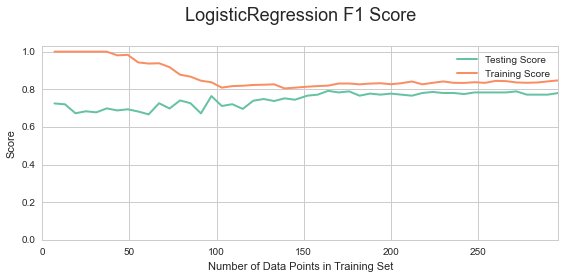
\includegraphics[width=0.75\textwidth]{figures/LogisticReg.png}
\caption{\label{fig:LogisticReg}Logistic Regression Learning Curve}
\end{figure}

\begin{table}[ht!]
\centering
\begin{tabular}{l|rrr}
{} & \multicolumn{3}{ c }{Training set size }         \\
{} &               103 &     200 &     296 \\\hline
prediction time (secs)   &            0.0868 &  0.0922 &  0.0662 \\
training time (secs)     &            0.0820 &  0.0889 &  0.0839 \\
F1 score on test set     &            0.7111 &  0.7770 &  0.7801 \\
F1 score on training set &            0.8088 &  0.8269 &  0.8474 \\
\end{tabular}
\caption{\label{tab:LogisticRegression}Logistic Regression Measurements}
\end{table}

% https://goo.gl/ICWc4P: shorthen for https://www.quora.com/What-are-the-advantages-of-logistic-regression-over-decision-trees
Some advantages\footnote{Source: \url{https://goo.gl/ICWc4P}} of Logistic Regression are that the model is fast, is less sophisticated and easy to inspect. Some of the downsides\footnote{Source: \url{http://d-scholarship.pitt.edu/7034/1/realfinalplus_ETD2006.pdf}} are are that, as any linear model, it is not robust to outliers, and can't handle imbalance data efficiently.


%%%%%%%%%%%%%%%%%%%%%%%%%%%%%%%%%%%%%%%%%%%%%%%%%%%%%%%%%%%%%%%%%%%%%%%%%%%%%%%%%%%%%%%%
%% CHOOSING THE BEST MODEL
%%%%%%%%%%%%%%%%%%%%%%%%%%%%%%%%%%%%%%%%%%%%%%%%%%%%%%%%%%%%%%%%%%%%%%%%%%%%%%%%%%%%%%%%

\section{Choosing the Best Model}
In this section, I will choose the model that best filled the requirements of limited resources and performance based on the experiments I have performed earlier. Thus, I will describe the algorithm in Layman's terms and, finally, tune it using Grid Search.

\subsection{Choosing the Optimal Model}
The $Logistic Regression$ model is the simplest of all algorithms tested and presented a remarkable performance, especially considering the imbalanced dataset used to train the model. Even this model had presented a performance similar to the other algorithm, it should be considered as the best one due to the Occam's Razor: "Among competing hypotheses, the one with the fewest assumptions should be selected".

Considering the time performance, the results of the $Logistic Regression$ was less stable than the other algorithms, when we look at the tables. For instance, the records show that it took $0.0992$ seconds to predict with 200 data points in the training set, against $0.0788$ of the $Decision Tree$ and $0.0801$ of the $GaussianNB$. However, the prediction time of the $Logistic Regression$ was the best one when used 296 data points. It dropped to $0.0662$ seconds to predict, against $0.0924$ from the $Decision Tree$ and $0.0890$ from the Naive Bayes. Overall, the time performance of the algorithm remained at an acceptable level, as can see in the Figure~\ref{fig:timetest}.

Comparing $Logistic Regression$ to $Decision Tree$, it has already achieved a $F_1$ score greater than $0.70$ using just 100 data point to fit the model, while the $Decision Tree$ took around 200 data point to achieve that. Comparing to $GuassianNB$, using 200 data points the Naive Bayes presented a $F_1$ score of $0.7111$. The $Logistic Regression$, $0.7770$. Also, it seems that this amount of data is enough for the model, given that adding more 96 data points just increased the $F_1$ score just $0.003$ units. 

\subsection{Describing the Model in Layman’s Terms}
As explained before, logistic regression is a classification method that performs a regression in a logistic function. It fits a model by calculating the maximum likelihood, using the conditional probability of G given X. In layman terms, it means that the model estimates its predictions\footnote{Source: \url{https://www.quora.com/What-is-logistic-regression}} using probability. The function approaches\footnote{Source: \url{https://www.quora.com/What-is-logistic-regression/answer/Alaka-Halder}} $0$ and $1$ asymptotically (after the required transformation), so the answer to the model always stay within the $[0,1]$ range. In the context of this project, $0$ means that the model is entirely sure that the student will fail to pass, and $1$ means that it is absolutely certain that student will pass. By default, any value above $0.5$ means that the model is pretty sure that the students will succeed, so it classifies as "passed."

\subsection{Model Tuning}
In this section, I performed a Grid Search through a parameter space looking for the set of parameters that yields the best result. This parameter space is all possible combinations of the following $Logistic Regression$ parameters:
\begin{itemize}
\item \textit{C}: [$0.01, 0.1, 0.5, 1., 2., 10., 100.$]
\item \textit{solver}: ['newton-cg', 'lbfgs', 'liblinear'] 
\end{itemize}

Where \textit{C} is the Inverse of regularization strength and \textit{solver} is the algorithm used in the optimization problem. To determine the "best result," Grid Search use a 3-fold Cross-validation procedure. Basically, it separates a sample into three subsets and uses one partition to train the model and another to verify its performance. Then, the procedure is run multiple times using different subsets to train and validate the model. The results are averaged over the rounds.

Calculating the F1 score using the classifier already tuned I got:

\begin{table}[ht]
\centering
\begin{tabular}{l|r}
 & Value \\\hline
Prediction time (secs) & 0.080 \\
Peak memory (MiB) & 97.92 \\
F1 score for training set & 0.826 \\
F1 score for test set & 0.787 \\
\end{tabular}
\caption{\label{tab:finalmodel}Final Model}
\end{table}

As was expected, after tuning the model, it performed just slightly better than the default parameters, achieving a $F_1$ score in the test set of $0.787$ against $0.7801$ obtained before. The prediction time got a little worse than before ($0.0662$).

%%%%%%%%%%%%%%%%%%%%%%%%%%%%%%%%%%%%%%%%%%%%%%%%%%%%%%%%%%%%%%%%%%%%%%%%%%%%%%%%%%%%%%%%
%% REFLECTION
%%%%%%%%%%%%%%%%%%%%%%%%%%%%%%%%%%%%%%%%%%%%%%%%%%%%%%%%%%%%%%%%%%%%%%%%%%%%%%%%%%%%%%%%

\section{Reflection}
Although I have found an appropriate model to the task at hand, I believe that I should have done some feature engineering or dimensionality reduction. I believe that the most of the models tested would benefit from a dataset with less dimensions. It would require the implementation of some new steps, including repeat what was done so far some more times gain. Running all the process, again and again, is expected. After all, as I have been learning at Udacity courses, Machine Learning can be very iterative.




\bibliographystyle{plain}
% or try abbrvnat or unsrtnat
\bibliography{bibliography/biblio.bib}
\end{document}
